% https://panthema.net/2013/0627-TikZ-Pythagoras-Tree/
% Draw Pythagoras Trees using TikZ
% Author: Timo Bingmann <tb@panthema.net>, 2013-06-27
\documentclass[a4paper]{article}

%\usepackage{fullpage}
\usepackage{tikz}
%\usepackage{animate}

% recursively draw a Pythagoras Tree fractal
% \PythagorasTree{levels}{angle}
\newcommand{\PythagorasTree}[2]{%
  \ifnum#1=0\else
    % randomly pick a color, prefer green and blue shades
    \pgfmathsetmacro{\r}{0.6*rnd}
    \pgfmathsetmacro{\g}{0.9*rnd}
    \pgfmathsetmacro{\b}{0.7*rnd}
    \definecolor{MyColor}{rgb}{\r,\g,\b}

    % draw the rectangle of this level
    \draw[draw=MyColor] (0,0) rectangle (1,1);

    % decrement level counter
    \pgfmathtruncatemacro{\next}{#1-1}

    % transform scope for left branch: move origin (1cm,0cm), rotate and scale
    % with the length of the left cathetus.
    \begin{scope}[
      yshift=1cm,xshift=0cm,
      rotate=#2,scale={cos(#2)}
      ]
      \PythagorasTree{\next}{#2}
    \end{scope}

    % now for the tricks: transform scope for right branch: move origin to the
    % top point of the triangle, rotate reverse and scale with length of right
    % cathetus.
    \begin{scope}[
      yshift={1cm * (1 + sin(#2)*cos(#2))},
      xshift={1cm * (cos(#2)*cos(#2))},
      rotate={#2-90},scale={sin(#2)}
      ]
      \PythagorasTree{\next}{#2}
    \end{scope}
  \fi
}

\begin{document}

\parindent=0pt

% draw just a single Pythagoras Tree
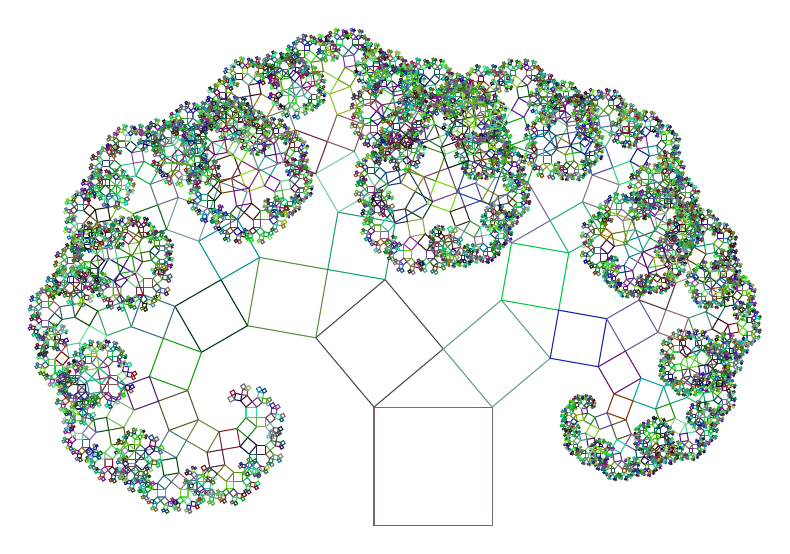
\begin{tikzpicture}[scale=1.5]
  % recursively draw tree
  \PythagorasTree{13}{40}
\end{tikzpicture}
% \bigskip\bigskip

% % macro to draw and annotate a Pythagoras Tree
% \newcommand{\MakeTree}[3]{%
%   % minipage to keep things together
%   \begin{minipage}{\linewidth}
%     \textbf{Pythagoras Tree, order #1, angle #2:}
%     \bigskip

%     \begin{center}
%       \begin{tikzpicture}[scale=1.5]
%         % recursively draw tree
%         \PythagorasTree{#1}{#2}
%         #3 % add some extra tikz code
%       \end{tikzpicture}
%     \end{center}
%     \bigskip

%   \end{minipage}
% }

% % draw some more trees with different parameters
% \iftrue
%   \MakeTree{13}{38}{}
%   \MakeTree{11}{45}{}
%   \MakeTree{11}{30}{}
%   \MakeTree{11}{65}{}
% \fi

% % draw animated growing Pythagoras Tree
% \iftrue
%   \clearpage
%   The following frame is an animated growing Pythagoras Tree, properly
%   viewable with Adobe Acrobat or other advanced PDF viewers:
%   \bigskip

%   \begin{animateinline}[autoplay,loop,controls,poster=last]{1}
%     \multiframe{13}{i=1+1}{
%       \MakeTree{\i}{40}{\useasboundingbox (-3,0) rectangle (3.5,4.5);}
%     }
%   \end{animateinline}
% \fi

\end{document}
%%% Local Variables:
%%% mode: latex
%%% TeX-master: t
%%% End:
